% !TEX root = ../main.tex
% =========================================================
% bab4.tex - HASIL DAN PEMBAHASAN
% Memerlukan tambahan paket: booktabs, pgfplots
% (lihat preambles_tambahan.tex).
% =========================================================

\chapter[HASIL DAN PEMBAHASAN]{\\ HASIL DAN PEMBAHASAN}

Bab ini memuat hasil pengolahan data pengujian kurva I--V modul PV
pasca-terendam beserta pembahasannya. Pembahasan disusun mulai dari
karakteristik data pengujian, kondisi pengukuran dan catatan irradiansi,
analisis status kelayakan berdasarkan $P_{max}$ STC, analisis deviasi parameter
terhadap \textit{nameplate}, analisis Fill Factor, analisis indikator $R_{VM}$
dan $R_{IM}$, interpretasi pola degradasi, serta implikasinya terhadap kegiatan
\textit{operation and maintenance}.

% ---------------------------------------------------------
\section{Karakteristik Data Pengujian}
% ---------------------------------------------------------

Data yang dianalisis terdiri dari 59 data pengujian kurva I--V. Data lengkap
hasil pengujian kurva I--V disajikan pada Lampiran~1, sedangkan bab ini hanya
memuat ringkasan parameter utama yang digunakan dalam analisis. Berdasarkan
keluaran perangkat lunak pengolah data, 6 data pengujian (10,17\%) memperoleh
status Ok, sedangkan 53 data pengujian (89,83\%) memperoleh status Not Ok.
Ringkasan status tersebut ditunjukkan pada Tabel~\ref{tab:status_pengujian}.
Status Ok/Not Ok merupakan hasil \textit{screening} performa daya oleh
perangkat lunak dan belum merepresentasikan keputusan akhir kelayakan
operasional.

\begin{table}[H]
\caption{Ringkasan status awal hasil pengujian modul PV}
\label{tab:status_pengujian}
\centering
\begin{tabular}{lcc}
\toprule
\textbf{Status} & \textbf{Jumlah Data} & \textbf{Persentase} \\
\midrule
Ok      & 6  & 10,17\%  \\
Not Ok  & 53 & 89,83\%  \\
\midrule
Total   & 59 & 100,00\% \\
\bottomrule
\end{tabular}
\end{table}

Distribusi $P_{max}$ STC dari seluruh data pengujian ditunjukkan pada
Gambar~\ref{gbr:dist_pmax}. Kelompok Ok terkonsentrasi pada kisaran 563--573~W,
sedangkan kelompok Not Ok berada pada kisaran 479--537~W. Rata-rata $P_{max}$
STC seluruh data adalah 508,47~W, sedangkan rata-rata kelompok Not Ok adalah
501,6~W.

\begin{figure}[H]
\centering
\begin{tikzpicture}
\begin{axis}[
    width=0.85\linewidth,
    height=0.30\textheight,
    xmin=460, xmax=590,
    ymin=0, ymax=21,
    xlabel={$P_{max}$ STC (W)},
    ylabel={Jumlah Data},
    grid=both,
    minor tick num=1,
    ybar,
    bar width=4pt,
    legend style={font=\scriptsize, at={(0.02,0.98)}, anchor=north west}
]
\addplot[fill=red!50, draw=red!80!black] coordinates {
    (475,1) (485,7) (495,15) (505,19) (515,6) (525,3) (535,2)
};
\addlegendentry{Not Ok}
\addplot[fill=blue!50, draw=blue!80!black] coordinates {
    (565,2) (575,4)
};
\addlegendentry{Ok}
\addplot[gray, dashed, no marks, line width=0.8pt] coordinates {(560,0) (560,21)};
\node[font=\scriptsize] at (axis cs:560,20.0) {Nominal 560 W};
\end{axis}
\end{tikzpicture}
\caption{Distribusi $P_{max}$ STC pada 59 data pengujian.}
\label{gbr:dist_pmax}
\end{figure}

% ---------------------------------------------------------
\section{Kondisi Pengukuran dan Catatan Irradiansi}
% ---------------------------------------------------------

Kondisi irradiansi saat pengukuran menjadi aspek penting dalam interpretasi
hasil. Tabel~\ref{tab:kondisi_irradiance} menunjukkan bahwa kelompok Ok diuji
pada irradiansi yang lebih rendah dibandingkan kelompok Not Ok. Perbedaan ini
perlu diperhatikan karena koreksi kurva I--V ke STC dari irradiansi rendah
dapat memiliki ketidakpastian yang lebih besar. Oleh sebab itu, status Ok
sebaiknya dikonfirmasi melalui pengujian ulang pada irradiansi yang lebih
representatif sebelum dijadikan dasar keputusan pemasangan kembali.

\begin{table}[H]
\caption{Ringkasan irradiansi pengujian pada setiap kelompok}
\label{tab:kondisi_irradiance}
\centering
\begin{tabular}{lcccc}
\toprule
\textbf{Kelompok} & \textbf{$n$} & \textbf{Min.} & \textbf{Maks.} &
\textbf{Rata-rata} \\
 & & \multicolumn{3}{c}{\textbf{Irradiansi \textit{Front} (W/m$^2$)}} \\
\midrule
Ok      & 6  & 198 & 265 & 232,8 \\
Not Ok  & 53 & 737 & 980 & 887,2 \\
\midrule
Total   & 59 & 198 & 980 & 820,6 \\
\bottomrule
\end{tabular}
\end{table}

% ---------------------------------------------------------
\section{Analisis Status Kelayakan Berdasarkan \texorpdfstring{$P_{max}$}{Pmax} STC}
% ---------------------------------------------------------

Status Ok dan Not Ok yang dihasilkan oleh perangkat lunak pengolah data
merupakan hasil \textit{screening} performa daya yang membandingkan $P_{max}$
STC terukur terhadap nilai \textit{nameplate} modul JKM560N-72HL4-BDV sebesar
560~W. Kelompok Ok memiliki rata-rata $P_{max}$ STC di atas nilai nominal,
sedangkan kelompok Not Ok memiliki rata-rata $P_{max}$ STC sebesar 501,6~W atau
sekitar 10,4\% di bawah nilai \textit{nameplate}. Penurunan tersebut
menunjukkan bahwa modul pada kelompok Not Ok mengalami penurunan performa daya
yang substansial terhadap spesifikasi pabrikan.

Status Not Ok tidak secara langsung menentukan jenis kerusakan fisik modul.
Keputusan pemasangan kembali tetap memerlukan pemeriksaan lanjutan, terutama
\textit{insulation resistance test} dan inspeksi visual, mengingat modul
memiliki riwayat terendam. Enam data Ok dapat dipertimbangkan sebagai kandidat
modul yang masih memenuhi kriteria performa daya, tetapi statusnya perlu
dikonfirmasi melalui pengujian ulang pada irradiansi yang lebih representatif
karena keenam data tersebut diperoleh pada irradiansi rendah (rata-rata
232,8~W/m$^2$).

% ---------------------------------------------------------
\section{Analisis Deviasi Parameter terhadap Nameplate}
% ---------------------------------------------------------

Deviasi parameter terhadap nilai \textit{nameplate} dihitung menggunakan
persamaan~\eqref{eq:deviasi_indikator}, dengan $X_{\text{ref}}$ adalah nilai
parameter pada \textit{datasheet} modul JKM560N-72HL4-BDV, yaitu
$P_{max,\text{ref}} = 560$~W, $V_{mp,\text{ref}} = 41{,}95$~V,
$I_{mp,\text{ref}} = 13{,}35$~A, $V_{oc,\text{ref}} = 50{,}67$~V, dan
$I_{sc,\text{ref}} = 14{,}13$~A. Deviasi ini menjadi dasar pembacaan arah
perubahan parameter elektrik pada masing-masing kelompok. Nilai positif
menunjukkan bahwa parameter terukur berada di atas nilai \textit{datasheet},
sedangkan nilai negatif menunjukkan penurunan terhadap referensi. Ringkasan
nilai rata-rata parameter dan deviasi terhadap \textit{datasheet} ditampilkan
pada Tabel~\ref{tab:deviasi}.

\begin{table}[H]
\caption{Perbandingan parameter rata-rata terhadap \textit{datasheet}}
\label{tab:deviasi}
\centering
\begin{tabular}{lccc}
\toprule
\textbf{Parameter} & \textbf{Datasheet} & \textbf{Ok} & \textbf{Not Ok} \\
\midrule
$P_{max}$ (W)         & 560   & 568,8      & 501,6      \\
$\Delta P_{max}$ (\%) & 0     & $+$1,6     & $-$10,4    \\
$V_{oc}$ (V)          & 50,67 & 52,03      & 49,59      \\
$\Delta V_{oc}$ (\%)  & 0     & $+$2,7     & $-$2,1     \\
$I_{sc}$ (A)          & 14,13 & 13,33      & 12,92      \\
$\Delta I_{sc}$ (\%)  & 0     & $-$5,6     & $-$8,5     \\
$V_{mp}$ (V)          & 41,95 & 44,92      & 40,40      \\
$\Delta V_{mp}$ (\%)  & 0     & $+$7,1     & $-$3,7     \\
$I_{mp}$ (A)          & 13,35 & 12,67      & 12,41      \\
$\Delta I_{mp}$ (\%)  & 0     & $-$5,1     & $-$7,0     \\
\bottomrule
\end{tabular}
\end{table}

Tabel~\ref{tab:deviasi} menunjukkan bahwa kelompok Ok memiliki $P_{max}$
rata-rata 568,8~W ($\Delta P_{max} = +1{,}6\%$), yang masih berada dalam
toleransi daya positif pabrikan. Sebaliknya, kelompok Not Ok memiliki $P_{max}$
rata-rata 501,6~W ($\Delta P_{max} = -10{,}4\%$). Parameter $V_{oc}$ pada
kelompok Ok berada di atas nilai \textit{datasheet}, sedangkan pada kelompok
Not Ok berada di bawahnya. Perbedaan yang lebih menonjol terlihat pada $V_{mp}$:
kelompok Ok memiliki rata-rata 44,92~V ($\Delta V_{mp} = +7{,}1\%$), sedangkan
kelompok Not Ok hanya 40,40~V ($\Delta V_{mp} = -3{,}7\%$). Penurunan $V_{mp}$
yang lebih besar dibandingkan penurunan $V_{oc}$ pada kelompok Not Ok
mengindikasikan bahwa perubahan performa lebih dominan terjadi pada sisi
tegangan operasi, terutama di sekitar titik daya maksimum. Sementara itu,
$I_{sc}$ dan $I_{mp}$ pada kedua kelompok sama-sama berada di bawah nilai
\textit{datasheet}, sehingga penurunan arus tidak sepenuhnya spesifik hanya
pada kelompok Not Ok. Deviasi ini selanjutnya digunakan sebagai dasar pembacaan
arah perubahan indikator $R_{VM}$ dan $R_{IM}$.

% ---------------------------------------------------------
\section{Analisis Fill Factor}
% ---------------------------------------------------------

Hasil perhitungan Fill Factor untuk seluruh data pengujian ditunjukkan pada
Gambar~\ref{gbr:ff_dist}. Nilai $FF$ referensi dari \textit{datasheet} adalah
0,7871, dihitung dari $P_{max}/(V_{oc}\cdot I_{sc}) = 560/(50{,}67\times14{,}13)$.

\begin{figure}[H]
\centering
\begin{tikzpicture}
\begin{axis}[
    width=0.85\linewidth,
    height=0.30\textheight,
    xmin=0, xmax=60,
    ymin=0.72, ymax=0.85,
    xlabel={Urutan Data Pengujian},
    ylabel={Fill Factor},
    grid=both,
    minor tick num=1,
    legend style={font=\scriptsize, at={(0.98,0.02)}, anchor=south east},
    only marks
]
\addplot[mark=*, mark size=1.5pt, blue!80!black] coordinates {
    (1,0.8100) (2,0.8300) (3,0.8300) (4,0.8200) (5,0.8100) (6,0.8100)
};
\addlegendentry{Ok}
\addplot[mark=triangle*, mark size=1.5pt, red!80!black] coordinates {
    (7,0.7900) (8,0.7900) (9,0.7800) (10,0.7900) (11,0.7800) (12,0.7800)
    (13,0.7800) (14,0.7800) (15,0.7800) (16,0.7800) (17,0.8000) (18,0.7800)
    (19,0.7800) (20,0.7800) (21,0.7700) (22,0.7800) (23,0.7900) (24,0.7900)
    (25,0.8000) (26,0.7800) (27,0.7900) (28,0.7700) (29,0.7800) (30,0.7900)
    (31,0.7800) (32,0.7800) (33,0.7800) (34,0.7800) (35,0.7900) (36,0.7800)
    (37,0.7800) (38,0.7900) (39,0.7900) (40,0.7700) (41,0.7800) (42,0.7700)
    (43,0.7700) (44,0.7900) (45,0.7900) (46,0.7900) (47,0.7700) (48,0.7900)
    (49,0.8000) (50,0.8000) (51,0.8000) (52,0.7900) (53,0.7700) (54,0.7900)
    (55,0.7900) (56,0.7800) (57,0.7900) (58,0.7900) (59,0.7300)
};
\addlegendentry{Not Ok}
\addplot[gray, dashed, no marks, line width=0.8pt, domain=0:60] {0.7871};
\node[font=\scriptsize] at (axis cs:50,0.7920) {$FF$ \textit{datasheet}};
\end{axis}
\end{tikzpicture}
\caption{Distribusi Fill Factor untuk 59 data pengujian.}
\label{gbr:ff_dist}
\end{figure}

Pada Gambar~\ref{gbr:ff_dist} terlihat bahwa kelompok Ok memiliki $FF$
rata-rata 0,818, sedangkan kelompok Not Ok memiliki $FF$ rata-rata 0,783. Nilai
rata-rata kelompok Not Ok berada sedikit di bawah nilai referensi
\textit{datasheet}, meskipun beberapa data Not Ok masih berada di sekitar nilai
referensi. $FF$ lebih tepat digunakan sebagai indikator perubahan bentuk kurva
I--V, bukan sebagai satu-satunya indikator kelayakan modul. Penurunan $FF$ pada
sebagian data Not Ok konsisten dengan kemungkinan peningkatan resistansi seri
($R_s$), degradasi kontak, korosi interkoneksi, atau mekanisme lain yang
menurunkan kualitas titik daya maksimum. Mekanisme fisik tersebut belum dapat
dipastikan hanya dari data I--V sehingga diperlukan pemeriksaan tambahan
seperti inspeksi visual, \textit{insulation resistance test}, termografi, atau
elektroluminesensi.

% ---------------------------------------------------------
\section{Analisis Indikator \texorpdfstring{$R_{VM}$}{RVM} dan \texorpdfstring{$R_{IM}$}{RIM}}
% ---------------------------------------------------------

Indikator $R_{VM}$ dan $R_{IM}$ dihitung untuk setiap data pengujian
menggunakan persamaan~\eqref{eq:rvm} dan \eqref{eq:rim}. Sebaran kedua
indikator pada bidang $R_{VM}$--$R_{IM}$ ditunjukkan pada
Gambar~\ref{gbr:scatter_rvm_rim}.

\begin{figure}[H]
\centering
\begin{tikzpicture}
\begin{axis}[
    width=0.85\linewidth,
    height=0.32\textheight,
    xmin=0.77, xmax=0.88,
    ymin=0.92, ymax=1.00,
    xlabel={$R_{VM} = V_{mp}/V_{oc}$},
    ylabel={$R_{IM} = I_{mp}/I_{sc}$},
    grid=both,
    minor tick num=1,
    legend style={font=\scriptsize, at={(0.02,0.02)}, anchor=south west},
    only marks
]
\addplot[mark=*, mark size=2pt, blue!80!black] coordinates {
    (0.8700,0.9350) (0.8637,0.9653) (0.8541,0.9716)
    (0.8654,0.9465) (0.8615,0.9426) (0.8646,0.9403)
};
\addlegendentry{Ok}
\addplot[mark=triangle*, mark size=1.6pt, red!80!black, opacity=0.7] coordinates {
    (0.8111,0.9699) (0.8124,0.9670) (0.8156,0.9546) (0.8134,0.9672)
    (0.8117,0.9613) (0.8247,0.9477) (0.8049,0.9696) (0.8167,0.9558)
    (0.8126,0.9587) (0.8216,0.9446) (0.8152,0.9828) (0.8160,0.9556)
    (0.8080,0.9686) (0.8303,0.9408) (0.8140,0.9420) (0.8140,0.9566)
    (0.8064,0.9818) (0.8147,0.9652) (0.8257,0.9696) (0.8000,0.9739)
    (0.8164,0.9656) (0.8147,0.9486) (0.8240,0.9513) (0.8350,0.9431)
    (0.8169,0.9552) (0.7980,0.9837) (0.8147,0.9552) (0.8000,0.9755)
    (0.8131,0.9673) (0.7948,0.9789) (0.8199,0.9556) (0.8140,0.9652)
    (0.8140,0.9652) (0.8124,0.9527) (0.8120,0.9636) (0.8163,0.9483)
    (0.8191,0.9462) (0.8206,0.9584) (0.8245,0.9521) (0.8182,0.9632)
    (0.8248,0.9355) (0.8093,0.9763) (0.8150,0.9768) (0.8167,0.9787)
    (0.8333,0.9560) (0.8296,0.9550) (0.8000,0.9635) (0.8316,0.9455)
    (0.8061,0.9773) (0.8145,0.9573) (0.8084,0.9722) (0.8258,0.9536)
    (0.7800,0.9359)
};
\addlegendentry{Not Ok}
\end{axis}
\end{tikzpicture}
\caption{Sebaran indikator $R_{VM}$ dan $R_{IM}$ untuk 59 data pengujian.}
\label{gbr:scatter_rvm_rim}
\end{figure}

Pada Gambar~\ref{gbr:scatter_rvm_rim} terlihat bahwa kelompok Ok terkonsentrasi
pada nilai $R_{VM}$ yang lebih tinggi, sedangkan kelompok Not Ok berada pada
rentang $R_{VM}$ yang lebih rendah. Rata-rata $R_{VM}$ kelompok Ok adalah
0,863, sedangkan kelompok Not Ok adalah 0,815. Sebaliknya, nilai $R_{IM}$ kedua
kelompok saling tumpang tindih, dengan rata-rata 0,950 pada kelompok Ok dan
0,961 pada kelompok Not Ok. Pola ini menunjukkan bahwa pemisahan kelompok
terutama terjadi pada sisi tegangan, konsisten dengan temuan pada
Tabel~\ref{tab:deviasi}.

Nilai referensi $R_{VM}$ dan $R_{IM}$ dihitung dari parameter \textit{datasheet}
modul JKM560N-72HL4-BDV:
\[
R_{VM,\text{ref}} = \frac{V_{mp,\text{ref}}}{V_{oc,\text{ref}}}
  = \frac{41{,}95}{50{,}67} = 0{,}828, \qquad
R_{IM,\text{ref}} = \frac{I_{mp,\text{ref}}}{I_{sc,\text{ref}}}
  = \frac{13{,}35}{14{,}13} = 0{,}945.
\]
Deviasi masing-masing indikator terhadap referensi dihitung menggunakan
persamaan~\eqref{eq:deviasi_indikator} dan dirangkum pada
Tabel~\ref{tab:rvm_rim_dev}.

\begin{table}[H]
\caption{Deviasi indikator $R_{VM}$ dan $R_{IM}$ terhadap nilai referensi
         \textit{datasheet}}
\label{tab:rvm_rim_dev}
\centering
\begin{tabular}{lccccc}
\toprule
\textbf{Indikator} & \textbf{Ref.} &
\textbf{Ok} & \textbf{Not Ok} &
\textbf{$\Delta$Ok (\%)} & \textbf{$\Delta$Not Ok (\%)} \\
\midrule
$R_{VM}$ & 0,828 & 0,863 & 0,815 & $+$4,23 & $-$1,57 \\
$R_{IM}$ & 0,945 & 0,950 & 0,961 & $+$0,55 & $+$1,71 \\
\bottomrule
\end{tabular}
\end{table}

Tabel~\ref{tab:rvm_rim_dev} menunjukkan bahwa $\Delta R_{VM}$ kelompok Not Ok
bernilai $-1{,}57\%$, artinya rasio tegangan operasi terhadap $V_{oc}$ menurun
terhadap nilai referensi. Sebaliknya, $\Delta R_{IM}$ kelompok Not Ok bernilai
$+1{,}71\%$ sehingga tidak menunjukkan penurunan pada sisi arus. Berdasarkan
persamaan~\eqref{eq:delta_v} dan \eqref{eq:delta_i}, diperoleh
$\delta_V = \max(0,\,1{,}57\%) = 1{,}57\%$ dan
$\delta_I = \max(0,\,-1{,}71\%) = 0{,}00\%$ untuk kelompok Not Ok. Indeks
dominasi dihitung menggunakan persamaan~\eqref{eq:dominasi_tegangan} dan
\eqref{eq:dominasi_arus}, dan hasilnya dirangkum pada
Tabel~\ref{tab:dominasi_penurunan}.

\begin{table}[H]
\caption{Indeks dominasi penurunan indikator sisi tegangan dan arus pada
         kelompok Not Ok}
\label{tab:dominasi_penurunan}
\centering
\begin{tabular}{lcccc}
\toprule
\textbf{Kelompok} & \textbf{$\delta_V$ (\%)} & \textbf{$\delta_I$ (\%)} &
\textbf{$D_V$} & \textbf{$D_I$} \\
\midrule
Not Ok & 1,57 & 0,00 & 1,00 & 0,00 \\
\bottomrule
\end{tabular}
\end{table}

Nilai $D_V = 1{,}00$ yang diperoleh pada Tabel~\ref{tab:dominasi_penurunan}
menunjukkan bahwa penurunan indikator yang terdeteksi lebih dominan terjadi
pada sisi tegangan. Hasil ini konsisten dengan $\delta_I = 0$ yang muncul
karena $\Delta R_{IM}$ kelompok Not Ok tidak bernilai negatif. Nilai $D_V$ yang
lebih besar menunjukkan bahwa penurunan indikator lebih dominan terjadi pada
sisi tegangan. Hasil ini tidak digunakan untuk menetapkan jenis gangguan secara
final, tetapi untuk membaca arah perubahan parameter elektrik pada kelompok Not
Ok.

Welch \textit{t-test} digunakan untuk membandingkan rata-rata parameter antara
kelompok Ok ($n=6$) dan kelompok Not Ok ($n=53$). Uji ini dipilih karena jumlah
data tidak seimbang dan variansi kedua kelompok tidak diasumsikan sama. Taraf
signifikansi yang digunakan adalah $\alpha=0{,}05$. Hasil uji berfungsi sebagai
pendukung interpretasi indikator, bukan sebagai dasar tunggal kelayakan
operasional.

Untuk setiap parameter $X \in \{P_{max},\,V_{oc},\,I_{sc},\,V_{mp},\,I_{mp},\,
R_{VM},\,R_{IM},\,FF\}$, hipotesis yang diuji adalah:
\begin{equation}
\begin{aligned}
H_0 &: \mu_{\mathrm{Ok},X} = \mu_{\mathrm{NotOk},X},\\
H_1 &: \mu_{\mathrm{Ok},X} \neq \mu_{\mathrm{NotOk},X},
\end{aligned}
\label{eq:hipotesis_welch}
\end{equation}
dengan $\mu_{\mathrm{Ok},X}$ adalah rata-rata parameter $X$ pada kelompok Ok
dan $\mu_{\mathrm{NotOk},X}$ pada kelompok Not Ok. Aturan keputusan dua arah
yang digunakan adalah:
\begin{equation}
p < \alpha \;\Rightarrow\; H_0 \text{ ditolak},\qquad
p \geq \alpha \;\Rightarrow\; H_0 \text{ tidak ditolak}.
\label{eq:keputusan_welch}
\end{equation}

Hasil pengujian ditunjukkan pada Tabel~\ref{tab:ttest}.

\begin{table}[H]
\caption{Hasil Welch \textit{t-test} antara kelompok Ok dan Not Ok}
\label{tab:ttest}
\centering
\begin{tabular}{lcccc}
\toprule
\textbf{Parameter} & \textbf{$t$} & \textbf{$p$-value} &
\textbf{Selisih Ok--Not Ok} & \textbf{Signifikan} \\
\midrule
$P_{max}$ & 26,95   & $<0,001$ & $+$13,4\% & Ya    \\
$V_{oc}$  & 20,13   & $<0,001$ & $+$4,9\%  & Ya    \\
$I_{sc}$  & 3,54    & 0,011    & $+$3,2\%  & Ya    \\
$V_{mp}$  & 27,09   & $<0,001$ & $+$11,2\% & Ya    \\
$I_{mp}$  & 4,15    & 0,001    & $+$2,0\%  & Ya    \\
$R_{VM}$  & 19,00   & $<0,001$ & $+$5,9\%  & Ya    \\
$R_{IM}$  & $-1,66$ & 0,150    & $-$1,1\%  & Tidak \\
$FF$      & 8,17    & $<0,001$ & $+$4,5\%  & Ya    \\
\bottomrule
\end{tabular}
\end{table}

Visualisasi signifikansi ditunjukkan pada Gambar~\ref{gbr:signifikansi_welch}
melalui nilai $-\log_{10}(p)$. Garis putus-putus pada $-\log_{10}(0{,}05)=1{,}301$
merupakan batas keputusan; batang yang melewati garis tersebut menunjukkan
parameter yang signifikan.

\begin{figure}[H]
\centering
\begin{tikzpicture}
\begin{axis}[
    width=0.82\linewidth,
    height=0.34\textheight,
    xbar,
    xmin=0, xmax=3.6,
    bar width=9pt,
    symbolic y coords={%
        $FF$,$R_{IM}$,$R_{VM}$,$I_{mp}$,$V_{mp}$,$I_{sc}$,$V_{oc}$,$P_{max}$},
    ytick=data,
    yticklabel style={font=\small},
    xlabel={$-\log_{10}(p)$},
    xmajorgrids=true,
    minor x tick num=1,
    enlarge y limits=0.12,
    extra x ticks={1.301},
    extra x tick labels={$\alpha{=}0{,}05$},
    extra x tick style={
        grid=major,
        grid style={dashed, gray!70, line width=0.9pt},
        tick label style={font=\scriptsize, gray!70, rotate=90, anchor=west},
        tick style={draw=none},
    },
    legend style={font=\scriptsize, at={(0.98,0.02)}, anchor=south east},
]
%--- Batang signifikan (biru) ---
\addplot[xbar, fill=blue!50, draw=blue!80!black] coordinates {
    (3.000,$P_{max}$)
    (3.000,$V_{oc}$)
    (1.959,$I_{sc}$)
    (3.000,$V_{mp}$)
    (3.000,$I_{mp}$)
    (3.000,$R_{VM}$)
    (3.000,$FF$)
};
\addlegendentry{Signifikan ($p<\alpha$)}
%--- Batang tidak signifikan (merah) ---
\addplot[xbar, fill=red!45, draw=red!80!black] coordinates {
    (0.824,$R_{IM}$)
};
\addlegendentry{Tidak signifikan ($p\geq\alpha$)}
\end{axis}
\end{tikzpicture}
\caption{Signifikansi parameter berdasarkan Welch \textit{t-test}.}
\label{gbr:signifikansi_welch}
\end{figure}

Berdasarkan persamaan~\eqref{eq:keputusan_welch} dan Gambar~\ref{gbr:signifikansi_welch},
hampir seluruh parameter berbeda signifikan antara kelompok Ok dan Not Ok,
kecuali $R_{IM}$ ($p=0{,}150\geq\alpha$, $H_0$ tidak ditolak). Indikator
$R_{VM}$ berbeda signifikan ($p<0{,}001$, $H_0$ ditolak), yang mendukung
interpretasi bahwa pemisahan kelompok lebih kuat terjadi pada sisi tegangan
daripada sisi arus. Hasil ini memperkuat temuan pada Tabel~\ref{tab:rvm_rim_dev}
dan konsisten dengan nilai $D_V=1{,}00$ pada Tabel~\ref{tab:dominasi_penurunan}.

% ---------------------------------------------------------
\section{Interpretasi Pola Degradasi}
% ---------------------------------------------------------

Berdasarkan hasil analisis deviasi, indikator $R_{VM}$/$R_{IM}$, indeks
dominasi, dan uji statistik, pola yang paling menonjol pada kelompok Not Ok
adalah penurunan sisi tegangan operasi. Penurunan $P_{max}$ rata-rata sebesar
10,4\% terhadap \textit{nameplate} diikuti oleh $\Delta R_{VM} = -1{,}57\%$
dan $D_V = 1{,}00$, yang menunjukkan bahwa arah penurunan indikator dominan
pada sisi tegangan. Indikator $R_{VM}$ berbeda signifikan antara kelompok Ok
dan Not Ok berdasarkan Welch \textit{t-test}, sedangkan $R_{IM}$ tidak berbeda
signifikan sehingga sisi arus bukan pemisah utama pada dataset ini. Interpretasi
ini dibatasi sebagai indikasi awal berbasis I--V dan tidak digunakan untuk
menetapkan jenis gangguan secara final.

Pola ini konsisten dengan kemungkinan peningkatan resistansi seri, degradasi
kontak, korosi interkoneksi, atau ketidakteraturan karakteristik sel yang
menyebabkan titik daya maksimum bergeser ke tegangan yang lebih rendah. Dalam
model satu dioda, peningkatan $R_s$ dapat menurunkan kualitas daerah
\textit{knee} kurva I--V dan berdampak pada penurunan $FF$
\cite{villalva2009}. Penurunan $I_{sc}$ pada kedua kelompok menunjukkan adanya
komponen penurunan pada sisi arus; akan tetapi, karena $R_{IM}$ tidak
menunjukkan perbedaan signifikan dan $\delta_I = 0$, penurunan arus tidak
menjadi indikator pemisah utama pada dataset ini.

Penyebab fisik degradasi belum dapat dipastikan hanya dari hasil pengujian I--V.
Riwayat perendaman membuat mekanisme berbasis kelembapan menjadi relevan untuk
dipertimbangkan, tetapi pembuktiannya tetap memerlukan data tambahan. Oleh
karena itu, hasil I--V pada analisis ini diposisikan sebagai dasar awal untuk
menentukan prioritas pemeriksaan lanjutan, bukan sebagai bukti tunggal
mengenai jenis kerusakan fisik modul.

% ---------------------------------------------------------
\section{Implikasi terhadap Operation and Maintenance}
% ---------------------------------------------------------

Pola degradasi yang teridentifikasi pada kelompok Not Ok memiliki implikasi
terhadap operasi sistem jika modul tersebut dipasang kembali pada
\textit{string}. Penurunan $V_{mp}$ pada modul Not Ok dapat memengaruhi
tegangan operasi \textit{string} jika modul tersebut tersusun seri dengan modul
lain yang masih normal. Tegangan operasi \textit{string} yang mengandung $N_d$
modul terdegradasi dapat dinyatakan seperti pada
persamaan~\eqref{eq:vstring_deg}.
\begin{equation}
V_{string,\text{deg}} =
\sum_{j=1}^{N_s-N_d} V_{mp,\text{normal}} +
\sum_{j=1}^{N_d} V_{mp,\text{deg}}
\label{eq:vstring_deg}
\end{equation}

Karena $V_{mp,\text{deg}} < V_{mp,\text{normal}}$, peningkatan jumlah modul
terdegradasi menurunkan tegangan operasi \textit{string}. Hasil I--V tidak
cukup untuk dijadikan dasar tunggal keputusan pemasangan kembali modul
pasca-terendam.

Modul-modul yang memperoleh status Not Ok perlu diprioritaskan untuk
pemeriksaan lanjutan sebelum keputusan pemasangan kembali diambil. Pengujian
tahanan isolasi (\textit{insulation resistance test}) menjadi prioritas karena
risiko utama pada modul pasca-terendam bukan hanya penurunan daya, tetapi juga
keselamatan listrik; paparan air dan kelembapan dapat menurunkan tahanan
isolasi dan meningkatkan risiko arus bocor atau \textit{ground fault}
\cite{ketjoy2022,smaGroundFault}. Untuk 6 data pengujian berstatus Ok, status
tersebut perlu dikonfirmasi melalui pengujian ulang pada irradiansi yang lebih
representatif, dan keputusan pemasangan kembali tetap memerlukan hasil
\textit{insulation resistance test} mengingat riwayat perendaman modul. Dengan
demikian, hasil I--V berfungsi sebagai dasar awal untuk memilah modul
berdasarkan performa daya, sedangkan keputusan operasional akhir harus
mempertimbangkan aspek keselamatan isolasi serta prosedur O\&M PLTS Terapung
Cirata.